\begin{itemize}

\item The self-energy flow is unreliable. It suffers from the finite frequency box of the vertex. 

\item Self energy inclusion suppresses the charge channel in favor of FM fluctuations, see FIg. \ref{selfsuppresfrg}. 

\item Self energy lowers the critical scale.

\item For the set of parameters consideresd ($U=4t$, $T=0.08t$, $t'=-0.10$, van Hove filling) the self energy seemed to be Fermi liquid like and did not show any sign of divergent behavior. 

\item In figure \ref{fermisurface} one can see that the self energy affects the Fermi surface which gets broadened, as we deduce from the momentum dependent occupation shown. 

\end{itemize}

\begin{figure}
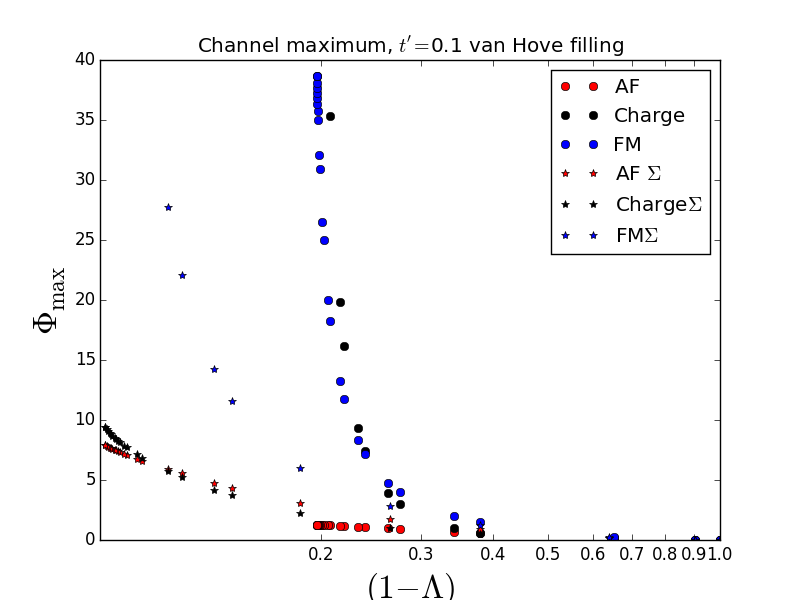
\includegraphics[scale=0.7]{images/sevsnose.png}
\caption{Max values of the channels as functions of cutoff scale, with and without self energy. }
\label{selfsuppressfrg}
 \end{figure}
 
 \begin{figure}
 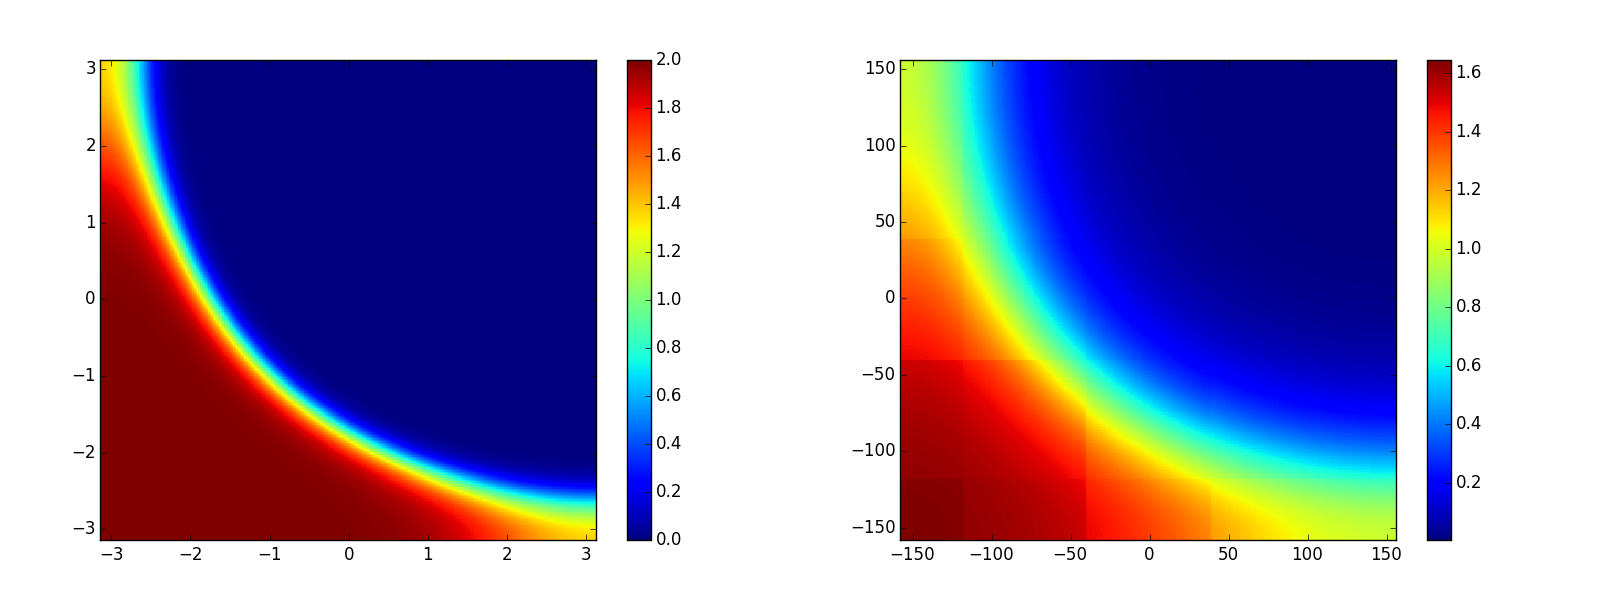
\includegraphics[scale=0.3]{images/Fermi_occupation_sevsnose.png}
 \caption{Occupation in the BZ: left non interacting, right with self energy from fRG.}
\label{fermisurface}
 \end{figure}
